%%%%%%%%%%%%%%%%%%%%%%%%%%%%%%%%%%%%%%%%%%%%%%%%%%%%%%%%%%%%%%%%%%%%%%%%%%%%%%%%
% TUM-Vorlage: Präsentation - Beispiele
%%%%%%%%%%%%%%%%%%%%%%%%%%%%%%%%%%%%%%%%%%%%%%%%%%%%%%%%%%%%%%%%%%%%%%%%%%%%%%%%

\begin{frame}
	\frametitle{CI/CD improvements}
	\begin{columns}
		\begin{column}{0.3\textwidth}
			\begin{figure}
				\centering
				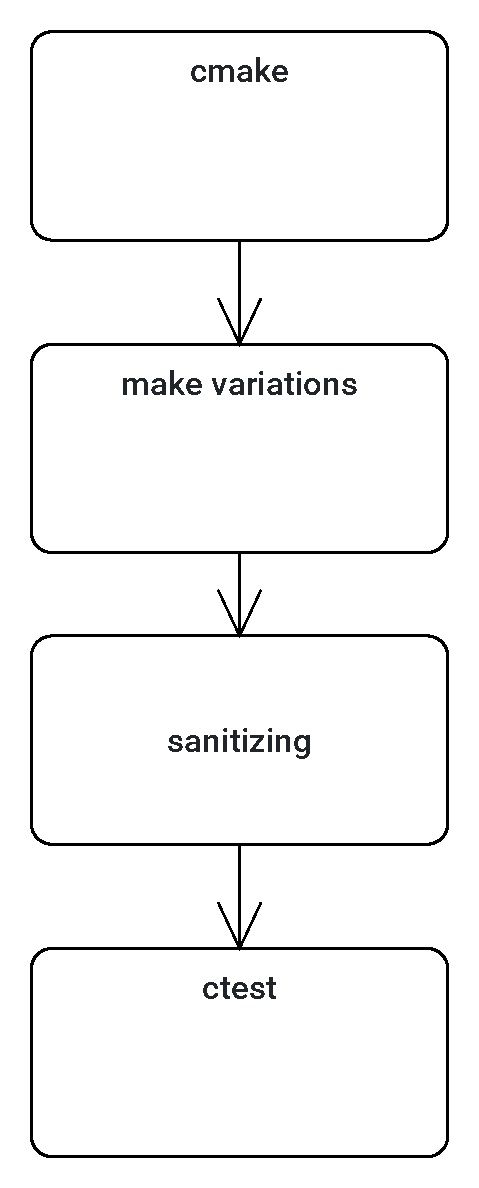
\includegraphics[width=0.55\linewidth]{cicd_old}
				\label{fig:cicdold}
			\end{figure}
			
		\end{column}
		
		\begin{column}{0.7\textwidth}
			\vspace{-1.5cm}
			\begin{figure}
				\centering
				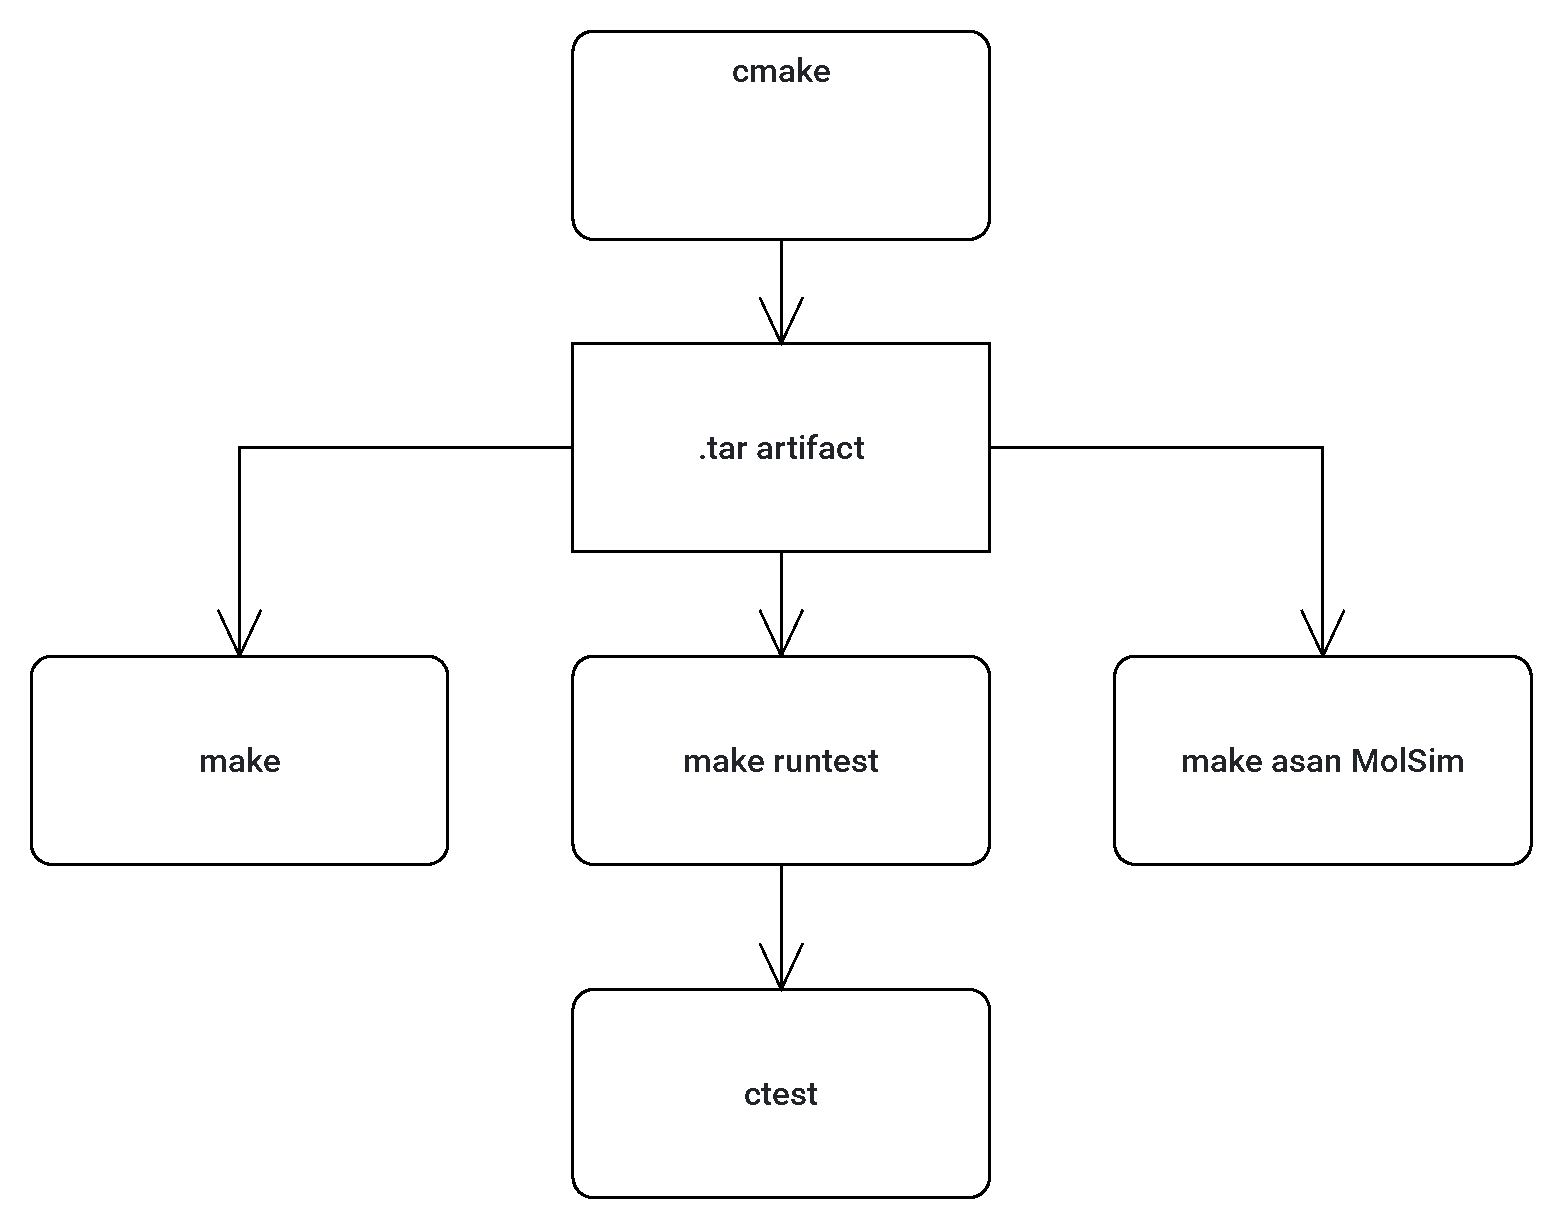
\includegraphics[width=0.8\linewidth]{cicd_new}
				\label{fig:cicdnew}
			\end{figure}
		\hspace{4cm}
		Reduced CI/CD time from 5m30s to 3m
			
		\end{column}
		
	\end{columns}
\end{frame}

\begin{frame}
	\frametitle{Thermostat}
	\begin{figure}
		\centering
		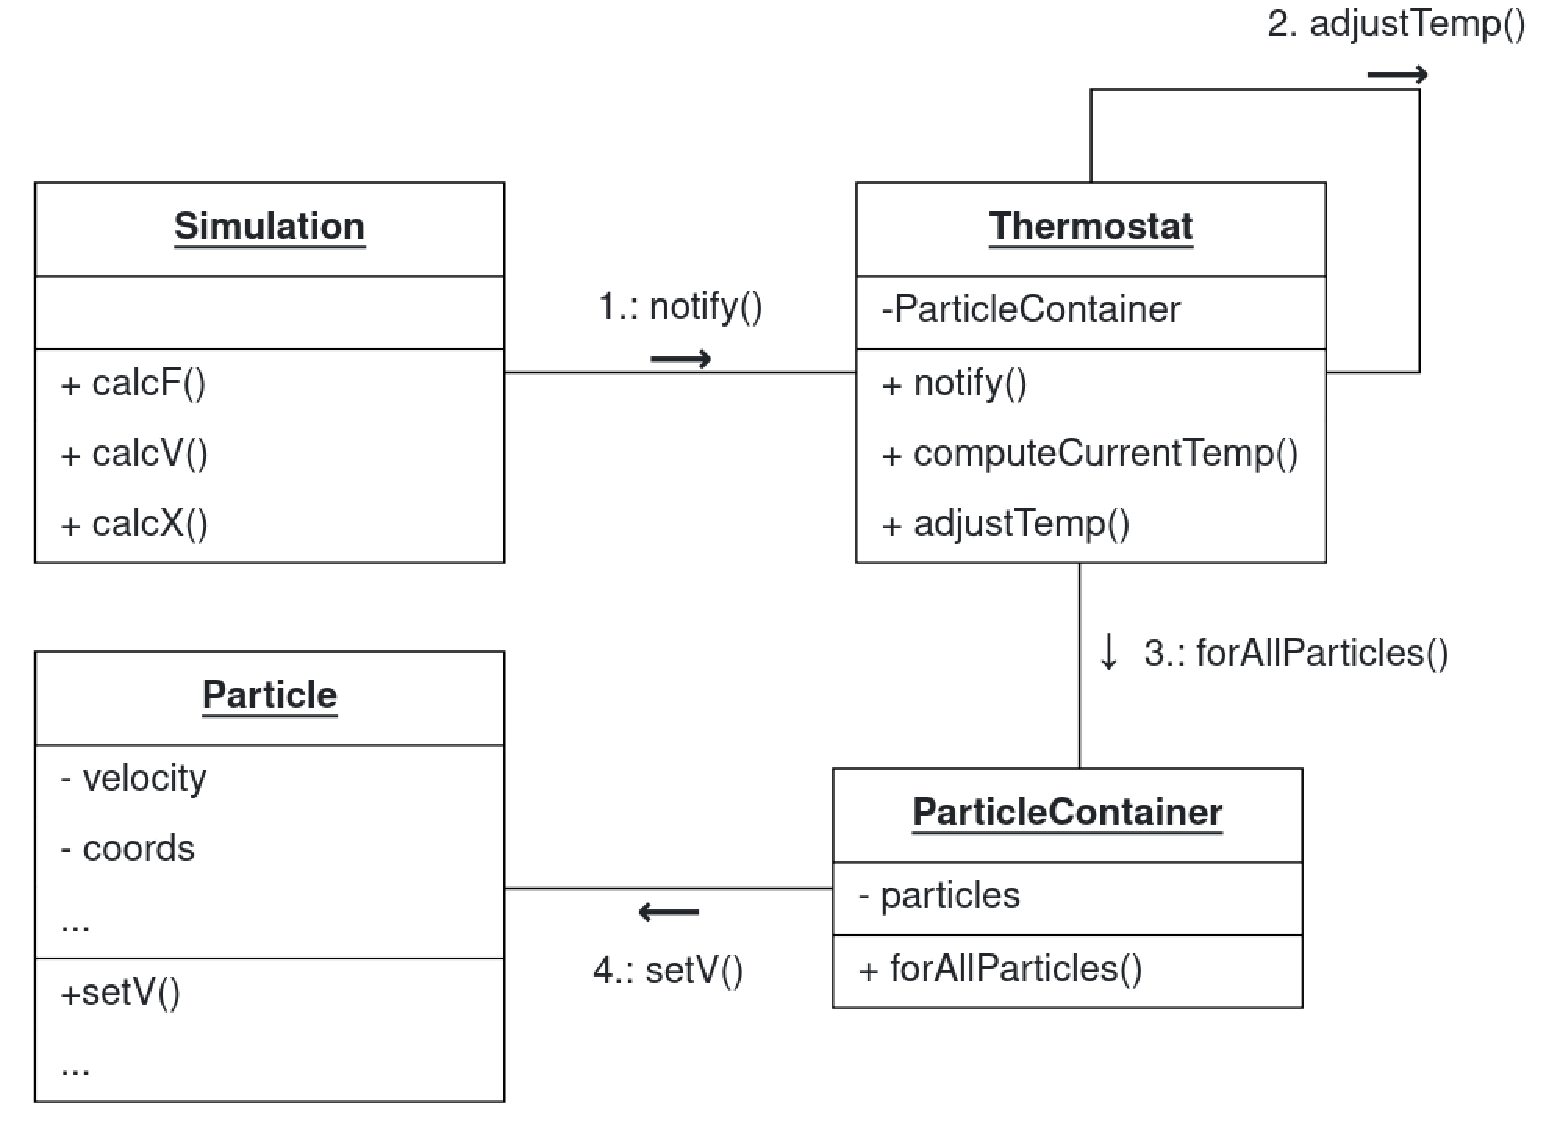
\includegraphics[width=0.55\linewidth]{ThermoComm}
		%\caption{}
		\label{fig:thermocomm}
	\end{figure}
	
	
\end{frame}

\begin{frame}
	\frametitle{Adapting ParticleContainer for periodic bounds}
	\large
	Idea:\\
	\begin{itemize}
		\item Provide virtual cells around the actual domain for anyone who needs it
		\item Existence of additional cells is invisible with old interface
	\end{itemize}
	
	\begin{columns}
		\begin{column}{0.6\textwidth}
			\vspace{-5cm}	
			\begin{figure}
				\centering
				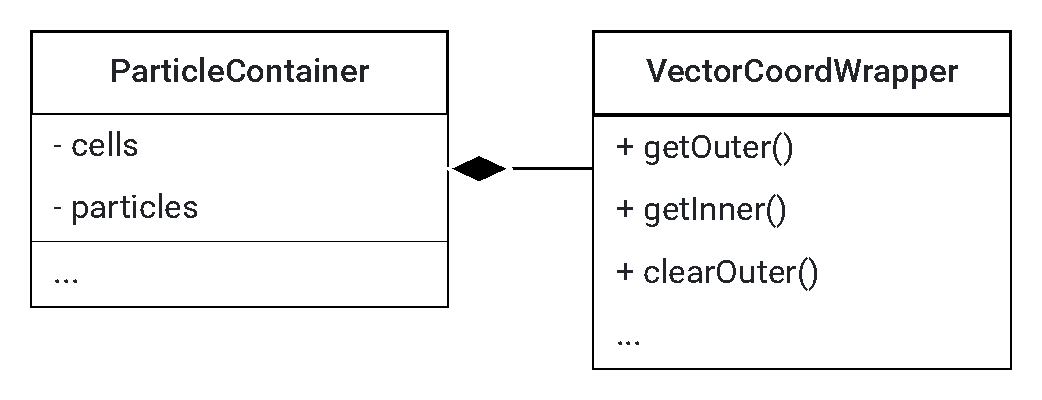
\includegraphics[width=\linewidth]{VectorCoordWrapper}
				\label{fig:vectorcoordwrapper}
			\end{figure}
		\end{column}
		
		\begin{column}{0.3\textwidth}
			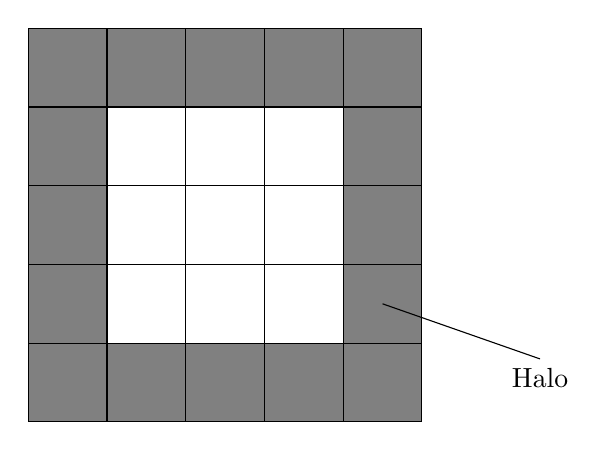
\begin{tikzpicture}
				\foreach \x in {1,...,3}{
					\foreach \y in {1,...,3}{
						\draw [draw=black] (\x, \y) rectangle (\x +1 ,\y + 1);
					}
				}
				\foreach \x in {0,...,4}{
					\filldraw [fill=gray, draw=black] (\x, 0) rectangle (\x +1 ,0 + 1);
					\filldraw [fill=gray, draw=black] (\x, 4) rectangle (\x+1, 4+1);
				}
			
				\foreach \y in {1,...,3}{
					\filldraw [fill=gray, draw=black] (0, \y) rectangle (0+1 , \y + 1);
					\filldraw [fill=gray, draw=black] (4, \y) rectangle (4+1, \y+1);
				}
			
				\draw [below] (4.5,1.5) -- (6.5, 0.8) node[below] {Halo};
			\end{tikzpicture}
		\end{column}
	\end{columns}


	
	
	
\end{frame}

\begin{frame}
\frametitle{Boundary conditions}
\large
Idea:
\vspace{-0.5cm}
\begin{enumerate}
	\item Temporarily move all particles next to Boundary of the other side
	\item Let Neighbouring cells interact
\end{enumerate} 

%\resizebox{0.5\textwidth }{0.5\textheight }{
	\begin{tikzpicture}[scale=1.3]
	%define constants
	\def\xLargeArrow{4.5}
	\def\yLargeArrow{1.5}
	\def\LargeArrowLength{2.5}
	\def\offSGrid{7.5}
	\def\arrowStart{0.6}
	\def\arrowEnd{1.9}
	
	\def\scale{1.4}
		
	%draw left grid
	\foreach \y in {0,...,2} {
		\filldraw [fill=green, draw=black] (0, \y) rectangle (0 + 1 ,\y + 1);
	}
	\foreach \x in {1,...,3}{
		\foreach \y in {0,...,2}{
			\draw [draw=black] (\x, \y) rectangle (\x +1 ,\y + 1);
		}
	}
	
	\fill (0.2,1.4) circle[radius=2pt];
	\fill (2.8,1.4) circle[radius=2pt];

	%arrow in between
	\draw[->, line width = 1mm] (\xLargeArrow, \yLargeArrow) -- (\xLargeArrow + \LargeArrowLength, \yLargeArrow);
	

	%draw right grid with left row put to the right
	\foreach \y in {0,...,2} {
		\filldraw [fill=green, draw=black] (\offSGrid + 3, \y) rectangle (\offSGrid + 3 + 1 ,\y + 1);
	}
	\foreach \x in {0,...,2}{
		\foreach \y in {0,...,2}{
			\draw [draw=black] (\offSGrid + \x, \y) rectangle (\offSGrid + \x +1 ,\y + 1);
		}
	}

	
	\fill (\offSGrid + 3 + 0.2,1.4) circle[radius=2pt];
	\fill (\offSGrid - 1 + 2.8,1.4) circle[radius=2pt];
	
	%arrows
	\draw[-triangle 60] (\offSGrid + 3.5, 1.5) -- (\offSGrid + 2.5, 1.5);
	\draw[-triangle 60] (\offSGrid + 3.5, 1.5) -- (\offSGrid + 2.5, 2.5);
	\draw[-triangle 60] (\offSGrid + 3.5, 1.5) -- (\offSGrid + 2.5, 0.5);
	
	
	\end{tikzpicture}
%}

\end{frame}

\begin{frame}
	\frametitle{The result}
	%TODO: insert video
	\begin{figure}[h!]
		\centering    
		\movie[label=show3,width=0.7\textwidth,poster
		,autostart,showcontrols,loop] 
		{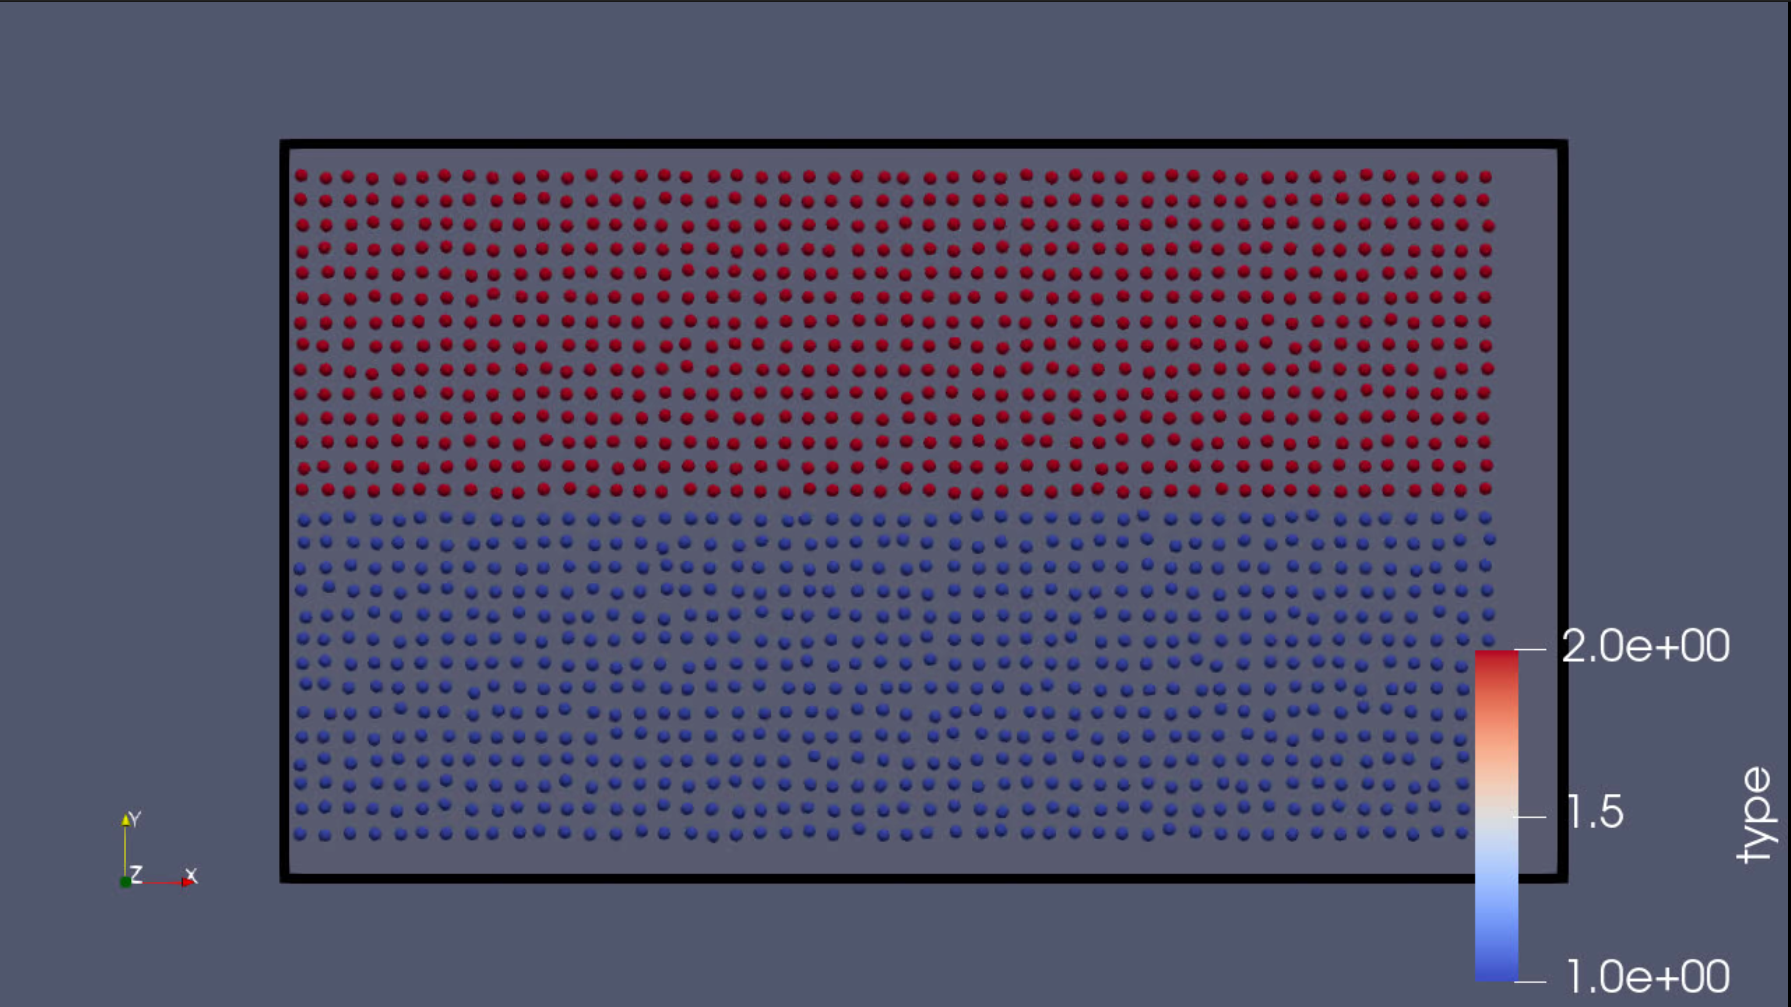
\includegraphics[width=0.7\textwidth]{small_rti.png}}{small_rti_broken.ogx}
		%\caption{caption}
	\end{figure} 
\end{frame}

\begin{frame}
	\frametitle{The problem}
	\large
	\begin{enumerate}
		\item Outer boxes may not have the expected sidelengths
		\item Interacting with neighbouring cells $\centernot \implies$ Catching everything in $r_{cutoff}$
	\end{enumerate}
	
			\begin{tikzpicture}[scale=1.3]
			%define constants
			\def\xLargeArrow{4.5}
			\def\yLargeArrow{1.5}
			\def\LargeArrowLength{2.5}
			\def\offSGrid{7.5}
			\def\arrowStart{0.6}
			\def\arrowEnd{1.9}
			
			\def\scale{1.4}
			
			%draw left grid
			\foreach \y in {0,...,2} {
				\filldraw [fill=green, draw=black] (0, \y) rectangle (0 + 1 ,\y + 1);
			}
			\foreach \x in {1,...,2}{
				\foreach \y in {0,...,2}{
					\draw [draw=black] (\x, \y) rectangle (\x +1 ,\y + 1);
				}
			}
			\foreach \y in {0,..., 2}{
				\draw [draw=black] (3, \y) rectangle (3 + 0.5,\y + 1);
			}
			
			\fill (0.2,1.4) circle[radius=2pt];
			\fill (2.8,1.4) circle[radius=2pt];
			
			%arrow in between
			\draw[->, line width = 1mm] (\xLargeArrow, \yLargeArrow) -- (\xLargeArrow + \LargeArrowLength, \yLargeArrow);
			
			
			%draw right grid with left row put to the right
			\foreach \y in {0,...,2} {
				\filldraw [fill=green, draw=black] (\offSGrid + 3 - 0.5, \y) rectangle (\offSGrid + 3 + 1 - 0.5,\y + 1);
			}
			\foreach \x in {0,...,1}{
				\foreach \y in {0,...,2}{
					\draw [draw=black] (\offSGrid + \x, \y) rectangle (\offSGrid + \x +1 ,\y + 1);
				}
			}
		
			\foreach \y in {0,..., 2}{
				\draw [draw=black] (\offSGrid + 2, \y) rectangle (\offSGrid + 2 + 0.5,\y + 1);
			}
			
			
			\fill (\offSGrid + 3 - 0.5 + 0.2,1.4) circle[radius=2pt];
			\fill (\offSGrid - 1 + 2.8,1.4) circle[radius=2pt];
			
			%arrows
			\draw[-triangle 60] (\offSGrid + 3.5 - 0.5, 1.5) -- (\offSGrid + 2.5 - 0.25, 1.5);
			\draw[-triangle 60] (\offSGrid + 3.5 - 0.5, 1.5) -- (\offSGrid + 2.5 - 0.25, 2.5);
			\draw[-triangle 60] (\offSGrid + 3.5 - 0.5, 1.5) -- (\offSGrid + 2.5 - 0.25, 0.5);
			
			
		\end{tikzpicture}
	
	$\implies$ Interact with one more "`Cellblock"' in that direction
\end{frame}

\begin{frame}
	\frametitle{Adding Periodic bounds}
	\large
	This slide should look very familiar to Assignment 3
		\begin{figure}
			\centering
			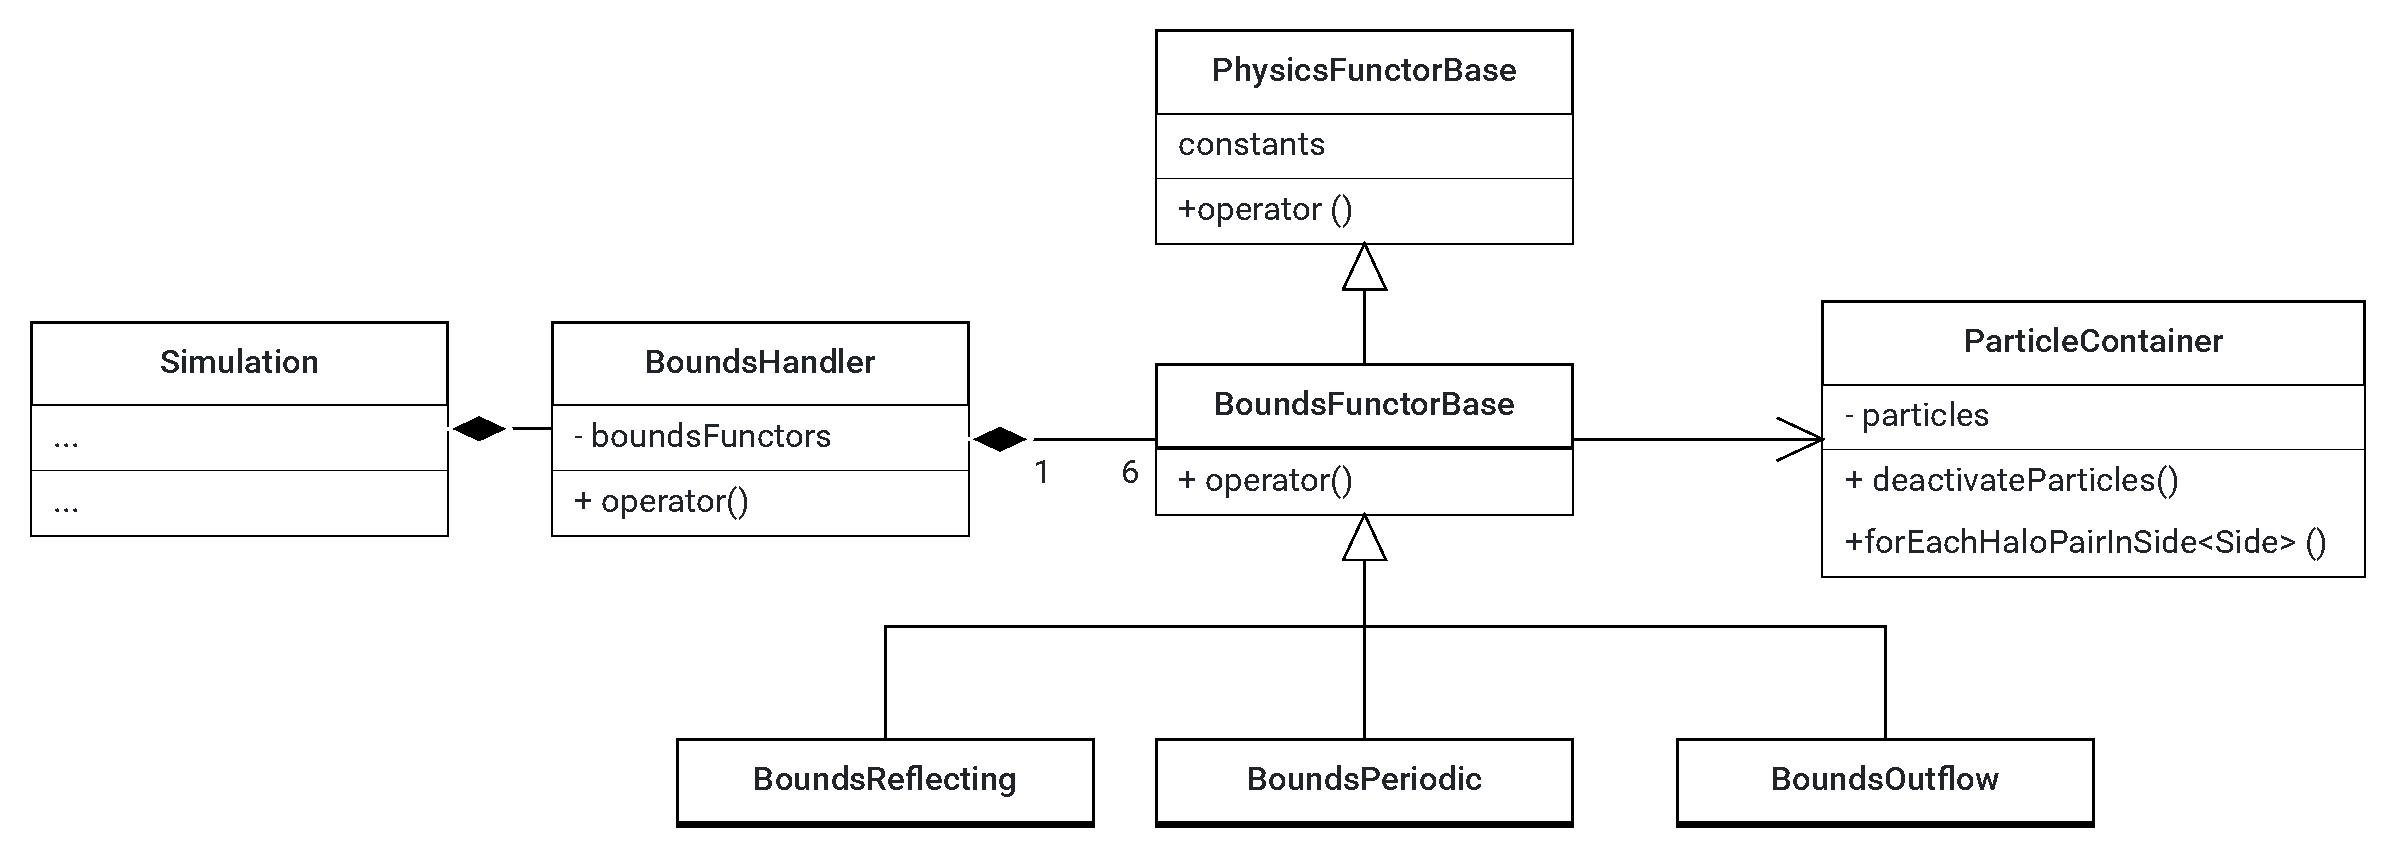
\includegraphics[width=0.95\linewidth]{BoundaryMolSim}
			\label{fig:boundarymolsim}
		\end{figure}
\end{frame}

\begin{frame}[fragile]
	\frametitle{Adding Gravitational Force}
	%\begin{columns}
	%	\begin{column}{0.5\textwidth}
			\begin{figure}
				\centering
				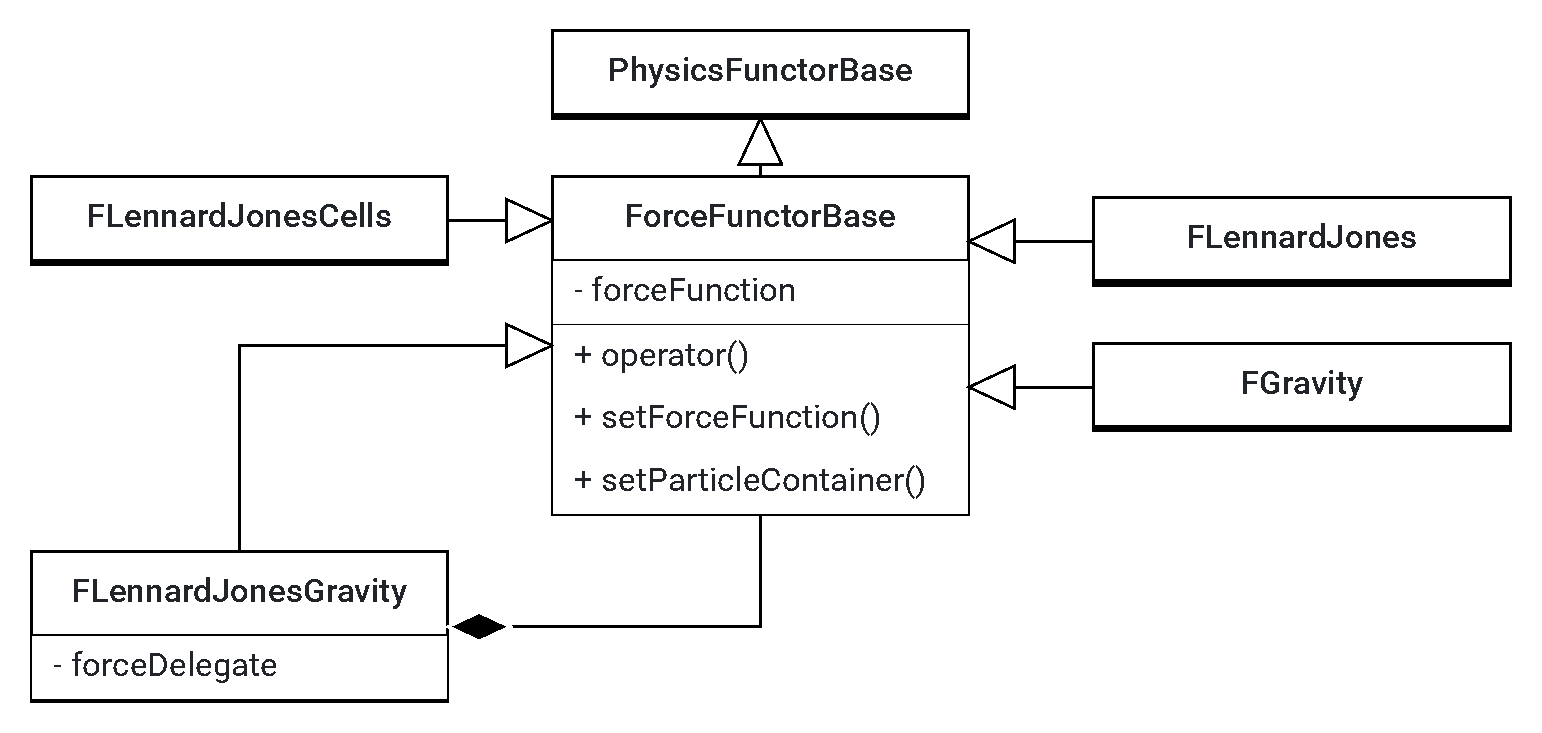
\includegraphics[width=0.6\linewidth]{FGravity_added}
				\label{fig:fgravityadded}
			\end{figure}
	%	\end{column}
	%\begin{column}{0.5\textwidth}
			
\begin{lstlisting}
		FLennardJonesGravity::operator()(){
			forceDelegate->operator()();
			particleContainer.forAllParticles([](auto& p){
			p.force[1] += p.m * gGrav;
			});	}
\end{lstlisting}

	%\end{column}
		
	%\end{columns}
	
\end{frame}

\begin{frame}[fragile]
	\frametitle{Optimizations 1}
	\large
As mentioned in Assignment 3 our ParticleContainer does not contain Particle-structs anymore.\\
Keeping the old interface lead to the following method:
\begin{lstlisting}
void ParticleContainer::forAllParticles(void(*function)(Particle &)) {
	for (unsigned long index: activeParticles) {
		Particle p;
		loadParticle(p, index);
		function(p);
		storeParticle(p, index);
	}
}
\end{lstlisting}

$\implies$ rewriting old code where this method got used was a major improvement

\end{frame}

\begin{frame}
	\frametitle{Optimizations 2}
	\large
	
	\begin{figure}
		\centering
		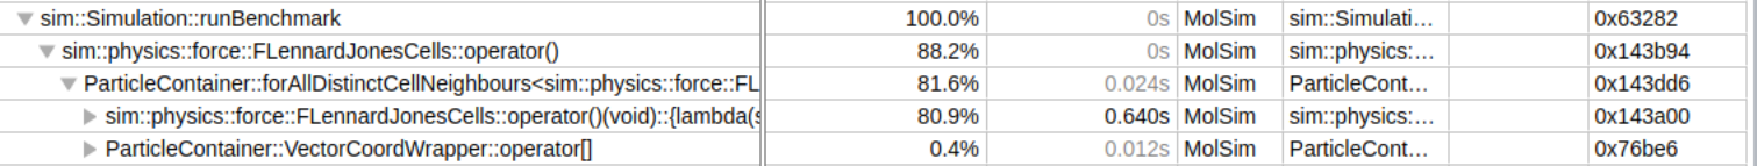
\includegraphics[width=1\linewidth]{profile_preoptimization_just_relevant_part}
		\label{fig:profilepreoptimizationjustrelevantpart}
	\end{figure}
	
	\begin{itemize}
		\item Force calculation takes a significant portion of CPU time
		\item Force between two particles in Force-Functors got represented as lambda expression
	\end{itemize}
	
	$\implies$ Represent force as static function instead
	
\end{frame}

\begin{frame}
	\frametitle{Small Rayleigh-Taylor instability}
	
	\begin{figure}[h!]
		\centering    
		\movie[label=show3,width=0.70\textwidth,poster
		,autostart,showcontrols,loop] 
		{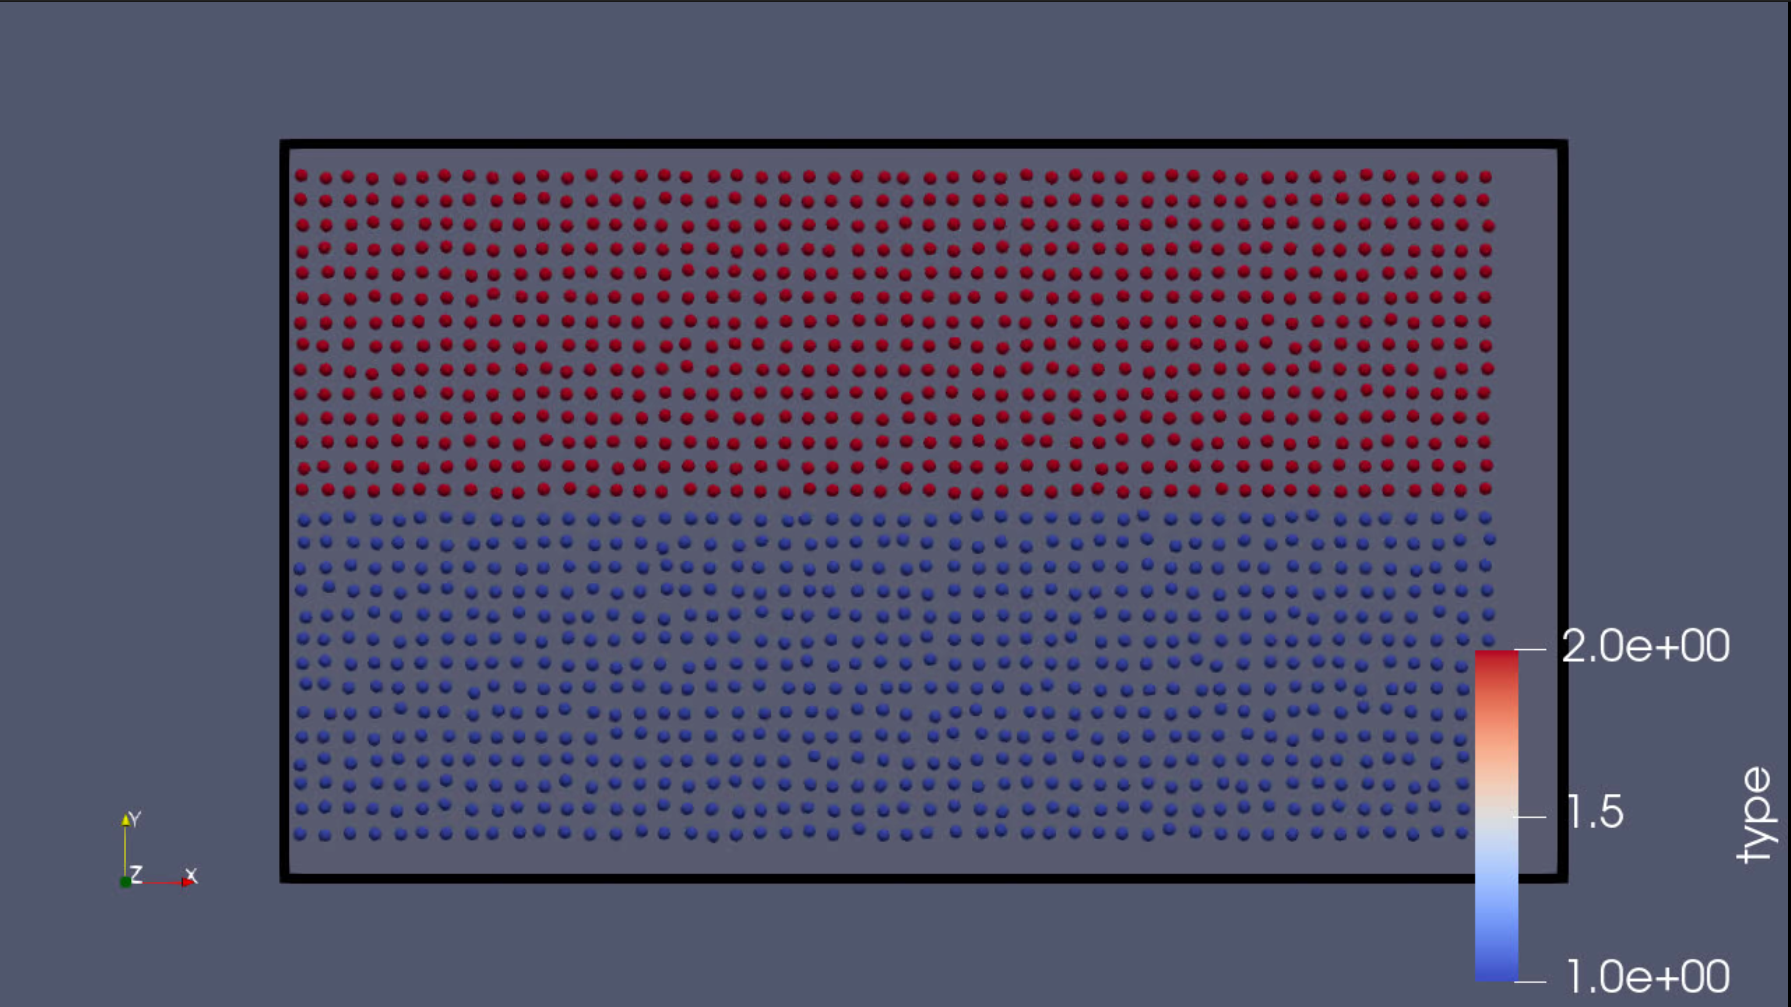
\includegraphics[width=0.70\textwidth]{small_rti.png}}{small_rti.mp4}
		%\caption{caption}
	\end{figure} 
	
\end{frame}

\begin{frame}
	\frametitle{Rayleigh-Taylor instability}
	\begin{figure}[h!]
		\centering    
		\movie[label=show3,width=0.75\textwidth,poster
		,autostart,showcontrols,loop] 
		{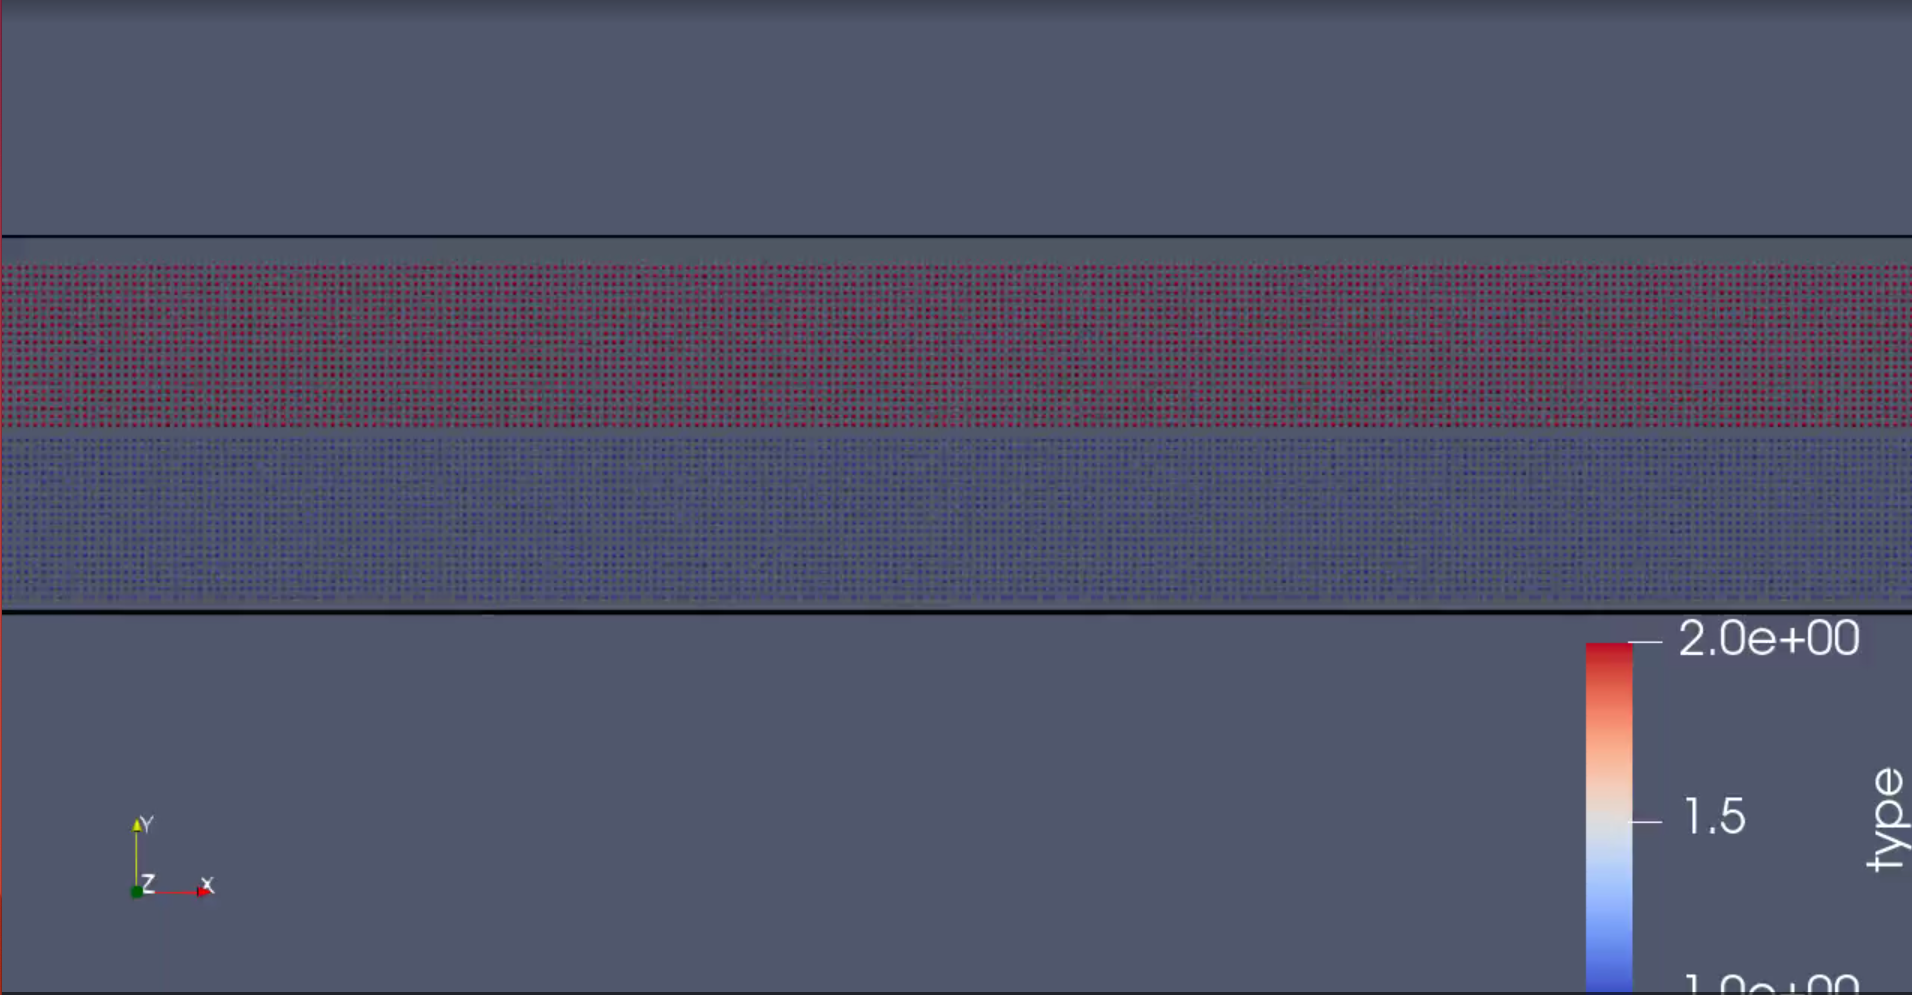
\includegraphics[width=0.75\textwidth]{large_rti.png}}{large_rti.mp4}
		%\caption{caption}
	\end{figure} 
\end{frame}

\begin{frame}
	\frametitle{Falling drop}
	\begin{figure}[h!]
		\centering    
		\movie[label=show3,width=0.70\textwidth,poster
		,autostart,showcontrols,loop] 
		{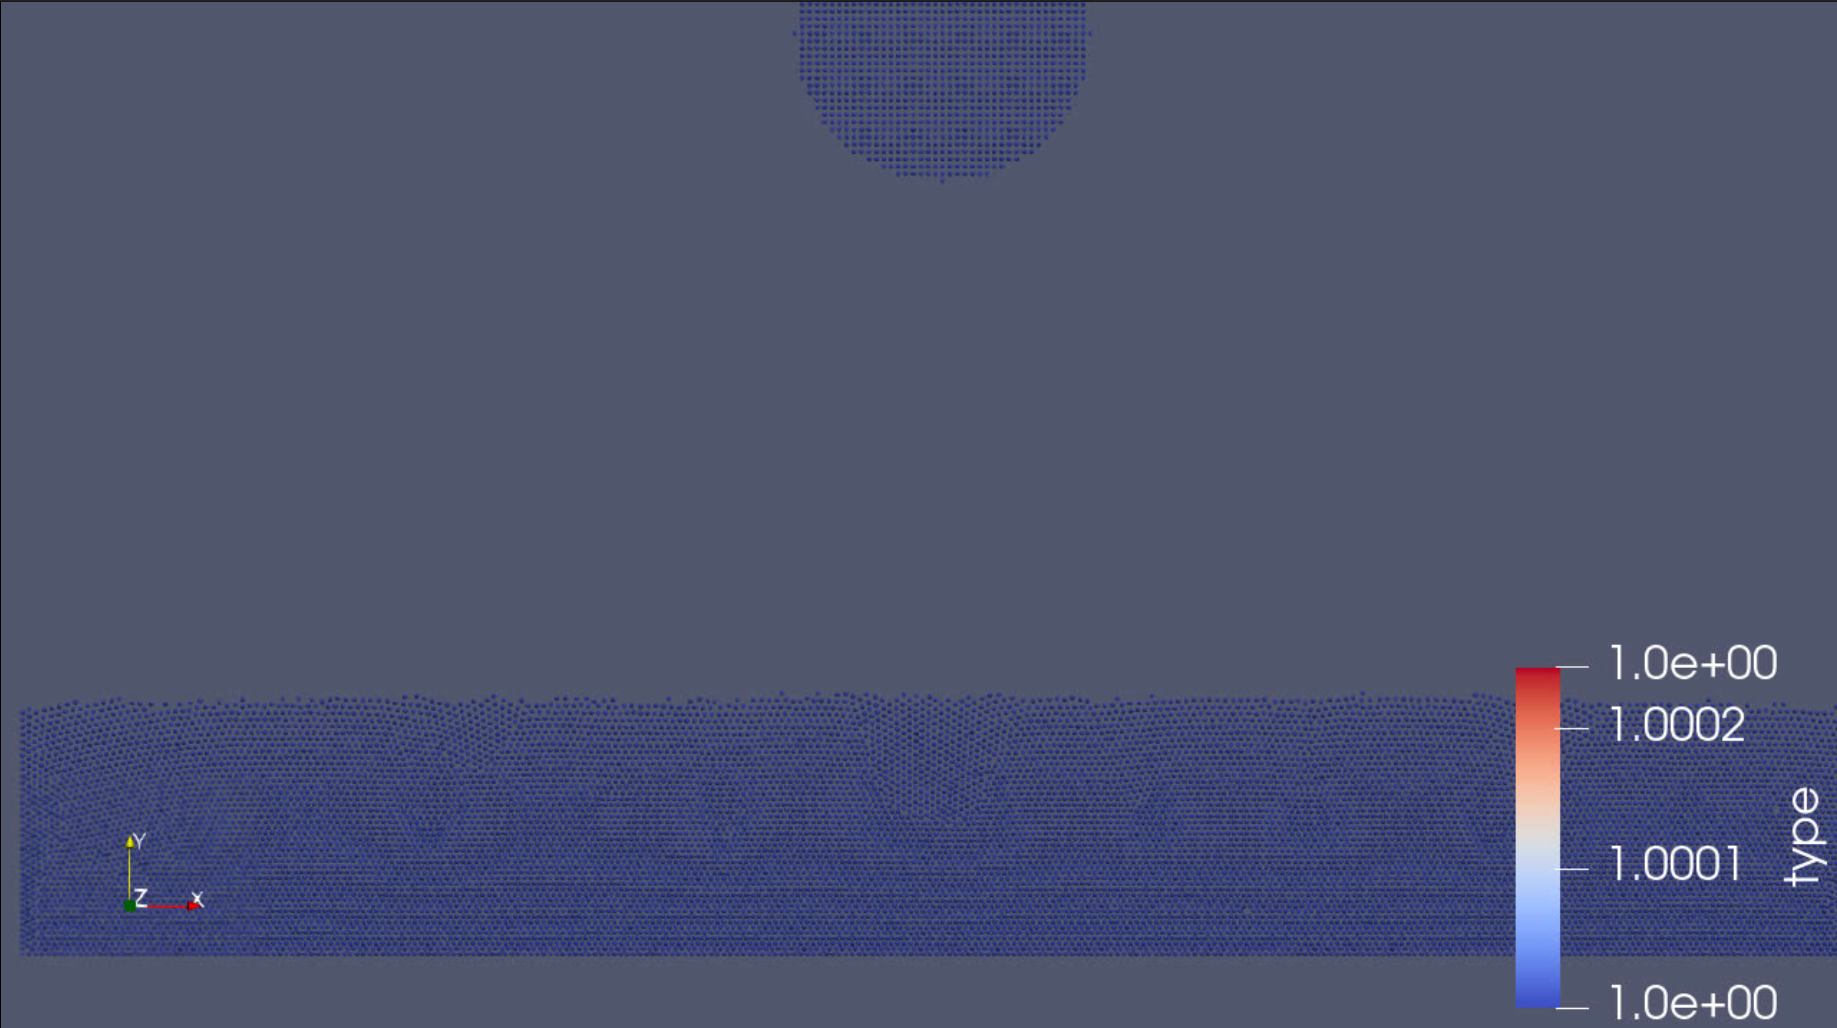
\includegraphics[width=0.70\textwidth]{falling_drop.png}}{falling_drop_out.mp4}
		%\caption{caption}
	\end{figure} 
\end{frame}

\begin{frame}
	\frametitle{Serial Benchmarks}
	\large
	\begin{itemize}
		\item As already mentioned building with the Intel compiled didn't work even with major time investments
		\item The option "`-slow"' lets the code run in the pre-optimized state
	\end{itemize}
	
	\Large
	\centering
	\begin{tabular}{lll}
		Options & MMU/s Cluster & MMU/s Local\\
		-slow -O2 & 0.0087 & \\
		-O2 & & 0.036\\
		-O0 & 0.0087 &\\	
	\end{tabular}

	\large
	Since these measurements smaller by orders of magnitude than our "`private test measurements"' and so close together we assume that something went wrong on the cluster.

\end{frame}

\begin{frame}
	\frametitle{Roadblocks}
	\large
	\begin{itemize}
		\item Compiling and running jobs on the cluster turned out to be a nightmare
		\item Intel compiler broke us trying to unbreak him
		\item Searching for bugs that may or may not be there (bouncy particles in Rayleigh-Taylor)
		\item Searching for bugs that definitely are there (see Boundary conditions)
		\item Large time investments in order to get tools to run
	\end{itemize}
\end{frame}

\begin{frame}
	\PraesentationBildUhrenturm
	%\PraesentationStartseiteFlaggen
\end{frame}

\begin{frame}
	\frametitle{Recreating Profiling}
	\large
	\begin{enumerate}
		\item \texttt{mkdir build}
		\item \texttt{cmake ..}
		\item \texttt{make ProfileMolSim} or \texttt{make CXX\_FLAGS+="-Dslow -std=c++20" ProfileMolSim}
		\item  \texttt{./ProfileMolSim ../input/[file\_you\_want\_to\_profile]}
		\item  \texttt{gprof ProfileMolSim gmon.out > profile-data.txt}
	\end{enumerate}
\end{frame}


%\frame[label=blah]{
%	\begin{center}%
%		\href{run:/usr/local/bin/mplayer -fs standard-benchmark.mp4}{
%		\includegraphics[scale=0.25]
%		{Assignment2_Presentation.pdf}}

%		\includemovie{.85\textheight}{.85\textheight}{standard-benchmark.mp4}%
%	\end{center}%
%	\note{%
%		\begin{itemize}
%			\item blah
%			\item blah
%		\end{itemize}
%	}%
%}


%%%%%%%%%%%%%%%%%%%%%%%%%%%%%%%%%%%%%%%%%%%%%%%%%%%%%
%% Folie: Gültigkeit der Masterfolien              %%
%%%%%%%%%%%%%%%%%%%%%%%%%%%%%%%%%%%%%%%%%%%%%%%%%%%%%
